\documentclass[a4paper]{article}
\usepackage[french]{babel}
%\usepackage[T1]{fontenc}
\usepackage[utf8]{inputenc}
\usepackage[figbotcap]{subfigure}  % use for side-by-side figures - ver  http://linuxdicas.wikispaces.com/latex
\usepackage{graphicx,amsmath,amssymb,algorithmic,algorithm,url,hyperref,tikz,enumitem,exam}
\usepackage[babel=true,kerning=true]{microtype} % <- bug labels tikz
\usetikzlibrary{arrows,shapes,snakes,automata,backgrounds,petri}

\graphicspath{{./},{../figures/},{../figures/automates/}}

\newtheorem{definition}{Définition}

\paper{IN310}
\school{ISAE - Supaero}
\subject{EXAMEN}
\title{Modèles de Systèmes Embarqués : modèles discrets, modèles hybrides}
\semester{3A SEM}
\year{2010-2011}
\note{Documents interdits. Des rappels de cours sont donnés à la fin de chaque partie.}

\begin{document}

%%%%%%%%%%%%%%%%%%%%%%%%%%%%%%%%%%%%%%%%%%
%%%%%%%%%%%% RESEAUX DE PETRI %%%%%%%%%%%%
%%%%%%%%%%%%%%%%%%%%%%%%%%%%%%%%%%%%%%%%%%

\exercice{Réseaux de Petri}

On modélise par le réseau de Petri de la figure \ref{petri} le fonctionnement d'un atelier qui doit réaliser deux types de pièces.
Pour le premier type de pièce, un opérateur doit placer la pièce dans une machine puis la retirer quand la machine a fini son travail.
Le deuxième type de pièce est traité de façon manuelle par un des deux opérateurs.

\begin{figure}[!h]
\begin{center}
	\begin{tikzpicture}[node distance=1.3cm,>=stealth',bend angle=45,auto]
	\tikzstyle{place}=[circle,thick,draw=blue!75,fill=blue!20,minimum size=6mm]
  	\tikzstyle{transition}=[rectangle,thick,draw=black!75,fill=black!20,minimum size=4mm]

    \node [transition] (t1) [label=above:$t_1$] {};
    \node [place] (p1) [below of=t1,label=left:$p_1$] {};
    \node [transition] (t2) [below of=p1,label=right:$t_2$] {};
    \node [place] (p2) [below of=t2,label=left:$p_2$] {};
    \node [transition] (t3) [below of=p2,label=right:$t_3$] {};
    \node [place] (p3) [below of=t3,label=left:$p_3$] {};
    \node [transition] (t4) [below of=p3,label=left:$t_4$] {};
    \node [place,tokens=1] (p4) [left of=p2,label=left:$p_4$] {};
    \node [place,tokens=2] (p5) [right of=p1,label=left:$p_5$] {};
    \node [place] (p6) [right of=p5,label=right:$p_6$] {};
    \node [transition] (t5) [above of=p6,label=right:$t_5$] {};
    \node [transition] (t6) [below of=p6,label=right:$t_6$] {};

	\draw (t1)
		edge [pre,bend left] (p5)
		edge [post] (p1);
	\draw (t2)
		edge [pre] (p1)
		edge [pre,bend right] (p4)
		edge [post] (p2)
		edge [post,bend right] (p5);
	\draw (t3)
		edge [pre] (p2)
		edge [pre] (p5)
		edge [post] (p3)
		edge [post,bend left] (p4);
	\draw (t4)
		edge [pre] (p3)
		edge [post,bend right] (p5);
	\draw (t5)
		edge [pre,bend right] (p5)
		edge [post] (p6);
	\draw (t6)
		edge [pre] (p6)
		edge [post,bend left] (p5);
	\end{tikzpicture}
	\caption{Réseau de Petri de l'atelier.}
	\label{petri}
\end{center}
\end{figure}

\begin{questions}
\question Donner la définition du réseau $R$ de la figure \ref{petri} ($P$, $T$, $Pre$ et $Post$) et son marquage initial $M_0$. \marks{1}

\begin{correction}{.8}
	$R = <P, T, Pre, Post>$ avec :
	\begin{eqnarray*}
	P &=& \{p_1, p_2, p_3, p_4, p_5, p_6\}\\
	T &=& \{t_1, t_2, t_3, t_4, t_5, t_6\}\\
	Pre &=& \begin{pmatrix}
	  % t1  t2  t3  t4  t5  t6
		0 & 1 & 0 & 0 & 0 & 0 \\ % p1
		0 & 0 & 1 & 0 & 0 & 0 \\ % p2
		0 & 0 & 0 & 1 & 0 & 0 \\ % p3
		0 & 1 & 0 & 0 & 0 & 0 \\ % p4
		1 & 0 & 1 & 0 & 1 & 0 \\ % p5
		0 & 0 & 0 & 0 & 0 & 1    % p6
		\end{pmatrix}\\
	Post &=& \begin{pmatrix}
	  % t1  t2  t3  t4  t5  t6
		1 & 0 & 0 & 0 & 0 & 0 \\ % p1
		0 & 1 & 0 & 0 & 0 & 0 \\ % p2
		0 & 0 & 1 & 0 & 0 & 0 \\ % p3
		0 & 0 & 1 & 0 & 0 & 0 \\ % p4
		0 & 1 & 0 & 1 & 0 & 1 \\ % p5
		0 & 0 & 0 & 0 & 1 & 0    % p6
		\end{pmatrix}\\
	M_0 &=& \begin{pmatrix} 0\\ 0\\ 0\\ 1\\ 2\\ 0\end{pmatrix}
	\end{eqnarray*}
\end{correction}

\question Donner la signification des six places du réseau $R$. \marks{2}

\begin{correction}{.8}
	\begin{itemize}
	\item $p_4$ et $p_5$ représentent les ressources disponibles :
		\begin{itemize}
		\item $p_4$ représente la disponibilité de la machine ;
		\item $p_5$ représente la disponibilité des opérateurs ;
		\end{itemize}
	\item $p_6$ représente le traitement d'une pièce de type 2 ;
	\item $p_1$, $p_2$ et $p_3$ représentent le traitement d'une pièce de type 1 :
		\begin{itemize}
		\item $p_1$ représente le placement de la pièce dans la machine,
		\item $p_2$ son traitement par la machine, et
		\item $p_3$ son retrait de la machine.
		\end{itemize}
	\end{itemize}
\end{correction}

\question Etudier les propriétés du réseau $R$ :
	\begin{enumerate}
	\item $R$ est-il borné ? Si oui, donner la valeur de la borne ; \marks{2}
	\item $R$ est-il vivant ? \marks{1}
	\item $R$ est-il réinitialisable ? \marks{1}
	\end{enumerate}
	
\begin{correction}{.8}
L'étude de ces propriétés peut se faire en calculant le graphe des marquages de $R$ depuis $M_0$.
Un modèle Tina (atelier.nd) est joint à ce corrigé afin de permettre de visualiser le graphe des marquages.
Dans ce cas ci, ce calcul peut être évité, en remarquant :
	\begin{enumerate}[leftmargin=1cm]
	\item que toute transition produit autant de jeton que ce qu'elle en consomme 
		($\forall t, \, Pre(.,t) = Post(.,t)$) ; donc il n'y aura jamais plus de 3 jetons dans ce réseau.
		$R$ est donc $k$-borné, avec $2 \leq k \leq 3$ ;
	\item que la séquence $M_0 \overset{t_1t_2t_1t_1}{\longrightarrow}$ mène à un blocage,
		aucune transition n'étant franchissable dans le marquage atteint ; le réseau n'est donc pas vivant ;
	\item et pour les mêmes raisons, le réseau n'est pas réinitialisable.
	\end{enumerate}
\end{correction}
	
\question Trouver au moins deux invariants de place du réseau. Que représentent-t-ils ? \marks{3}

\begin{correction}{.8}
Soit $f_1 = \begin{pmatrix} 1 & 0 & 1 & 0 & 1 & 1\end{pmatrix}$,
\begin{eqnarray*}
f_1 . C &=& f_1 . (Post - Pre)\\
	&=& \begin{pmatrix} 1 & 0 & 1 & 0 & 1 & 1\end{pmatrix} . \begin{pmatrix}
	  % t1  t2  t3  t4  t5  t6
		1 & -1 & 0 & 0 & 0 & 0 \\ % p1
		0 & 1 & -1 & 0 & 0 & 0 \\ % p2
		0 & 0 & 1 & -1 & 0 & 0 \\ % p3
		0 & -1 & 1 & 0 & 0 & 0 \\ % p4
		-1 & 1 & -1 & 1 & -1 & 1 \\ % p5
		0 & 0 & 0 & 0 & 1 & -1    % p6
		\end{pmatrix}\\
	&=& \begin{pmatrix} 0 & 0 & 0 & 0 & 0 & 0\end{pmatrix}
\end{eqnarray*}
$f_1$ est donc une composante conservative, et $\forall M, \, f_1 . M = f_1 . M_0 = 2$.
Cet invariant de place représente le fait qu'il y a toujours 2 opérateurs dans l'atelier, occupés à diverses tâches.\\

Soit $f_2 = \begin{pmatrix}0 & 1 & 0 & 1 & 0 & 0\end{pmatrix}$, $f_2 . C = 0 $, $f_2$ est donc une 
composante conservative, et $\forall M, \, f_2 . M = f_2 . M_0 = 1$.
Cet invariant de place représente le fait que la machine est soit disponible, soit occupée par une pièce.\\

$R$ est complètement couvert par les composantes $f_1$ et $f_2$, $R$ est donc borné, et ça borne vaut $2$.
\end{correction}

\end{questions}


%%%%%%%%%%%%%%%%%%%%%%%%%%%%%%%%%%%%%%%%%%
%%%%%%%%%%%% AUTOMATES %%%%%%%%%%%%%%%%%%%
%%%%%%%%%%%%%%%%%%%%%%%%%%%%%%%%%%%%%%%%%%
\newpage
\exercice{Automates}

\begin{questions}
\question \textbf{Équivalence pour des systèmes : } Rappeler, à l'aide d'un exemple, en quoi l'équivalence de traces n'est
	pas toujours suffisante pour comparer deux systèmes.\\
	\emph{Réponse de 5 lignes maximum + un dessin éventuellement}
\marks{2}

\begin{correction}{.8}
  L'équivalence de traces ne prend pas en compte le branchement, c'est
  à dire la prise en compte de différentes manières de poursuivre
  l'exécution depuis un état donné. Dans l'exemple suivant, les deux
  automates $\mathcal{A}_1$ et $\mathcal{A}_2$ sont équivalents au
  sens de l'équivalence de traces, mais mis en présence de $\mathcal{B}$,
  $\mathcal{A}_1||\mathcal{B}$ ne possède pas de deadlock, alors que
  $\mathcal{A}_2||\mathcal{B}$ si.
\begin{center}
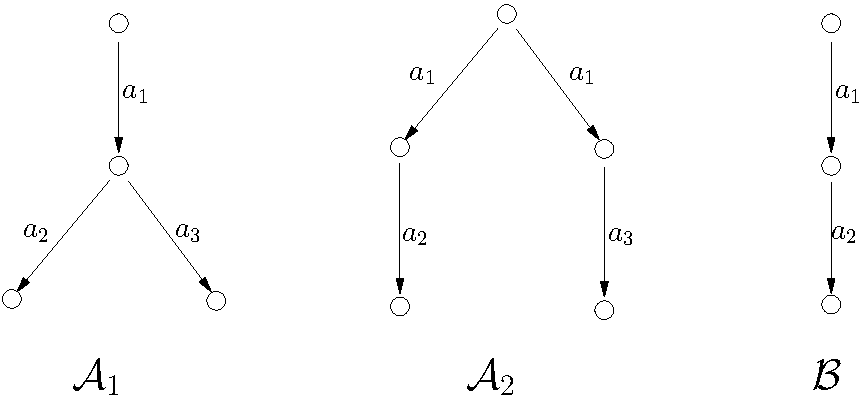
\includegraphics[width=6cm]{equiv_traces}
\end{center}
\end{correction}

\question \textbf{Automates temporisés : } Considérons l'automate
temporisé de la figure \ref{automateT} sur l'alphabet (ensemble de
labels) $\Sigma=\{a_1,a_2,a_3\}$, comportant une horloge $x$. Donner,
sans justification, deux exemples de traces temporisées reconnues par
cet automate. (Donner des séquences sur $\Sigma \times \mathbb{R}_+$,
c'est à dire des séquences de paires (\texttt{label}, \texttt{durée
  d'attente})). \marks{2}
	\begin{figure}[!h]
		\begin{center}
		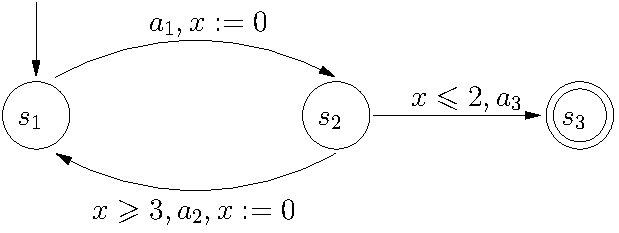
\includegraphics[width=6cm]{automate_temp}
		\end{center}
		\caption{Automate temporisé.}
		\label{automateT}
	\end{figure}

\begin{correction}{.8}
Deux traces acceptées par l'automate:\\
$(a_1,3);(a_3,1.2)$\\
$(a_1,4.1);(a_2,3.3);(a_1,3.1);(a_3,1.5)$
\end{correction}

        \question La sémantique d'un automate temporisé est donnée par
        un système de transitions temporisé, dont l'espace d'état est
        infini.  Rappeler les grandes idées de la construction d'un
        système de transitions fini (qui permet donc de vérifier
        certaines propriétés)
	<<équivalent>> au système de transition temporisé infini. Dans quel sens est-il équivalent?\\
	\emph{Réponse de 10 lignes maximum } \marks{3}

\begin{correction}{.8}
L'ensemble des configurations d'un automate temporisé est infini à
cause du domaine des horloges ($\mathbb{R}_+$). L'idée est de
construire un ensemble fini de régions pour chaque horloge, telle que
quelle que soit la valeur d'une horloge dans une région, l'état du
système soit inchangé (les mêmes invariants et gardes sont
satisfaits). Une configuration du système abstrait peut alors être donnée par
un couple (localité, région) plutôt que (localité, valeur des
horloges). Ce système abstrait est en relation de bisimulation
temps-abstraite avec le système d'origine, ce qui garantit qu'il
satisfait les mêmes propriétés.
\end{correction}

\question Soient $T=(S,S_I,S_F,\rhd )$ et $T'=(S',S'_I,S'_F,\rhd')$ deux systèmes de transitions temporisés. Si $\mathcal{R}$ est une
	relation de bisimulation temps-abstraite qui respecte l'état
        initial et l'état final, montrer que \linebreak
        Untime(L(T))=Untime(L(T')). \marks{3}
\end{questions}

\begin{correction}{.8}
Soit $(a_1,\ldots, a_n)\in Untime(L(T))$. 
$\exists (t_1,\ldots , t_n), \exists (s_1,\ldots,s_{n+1})$ tels que
$s_1\overset{t_1,a_1}{\rhd}s_2 \overset{t_2,a_2}{\rhd} \ldots
\overset{t_n,a_n}{\rhd}s_{n+1}$ et $s_{n+1}\in S_F$. 

Montrons par récurrence sur $k$ que $\forall k\in [|1..n+1|] \exists
t'_k,s'_k,s'_{k+1}$ tels que $s_k\mathcal{R} s'_k$,
$s_{k+1}\mathcal{R} s'_{k+1}$, et $s'_k\overset{t'_k,a_k}{\rhd}s'_{k+1}$.

$\bullet$ $\mathcal{R}$ étant une relation de bisimulation, l'hypothèse est
trivialement vérifiée au rang 1.
 
$\bullet$ Supposons l'hypothèse de récurrence vraie au rang k. Alors, on a
$s_{k+1}\mathcal{R} s'_{k+1}$. Par ailleurs,
$s_{k+1}\overset{t_{k+1},a_{k+1}}{\rhd}s_{k+2}$. Puisque $\mathcal{R}$ est une
bisimulation temps-abstraite, $\exists t'_{k+1}, s'_{k+1}$ tels que
$s_{k+2}\mathcal{R}s'_{k+2}$ et  $s'_{k+1}\overset{t'_{k+1},a_{k+1}}{\rhd}s'_{k+2}$.
Donc l'hypothèse de récurrence est vraie au rang k+1.

On a donc prouvé qu'il existe $(s'_1, \ldots, s'_{n+1})$ et
$(t'_1,\ldots , t'_n)$ et tels que $s'_1\overset{t'_1,a_1}{\rhd}s'_2
\overset{t'_2,a_2}{\rhd} \ldots \overset{t'_n,a_n}{\rhd}s'_{n+1}$. De
plus, puisque $\mathcal{R}$ respecte les états initiaux et finaux,
$s'_1\in S'_I$, $s'_{n+1}\in S'_F$. Donc $(a_1,\ldots, a_n)\in
Untime(L(T'))$.

De manière symétrique, on peut prouver que  $Untime(L(T')) \subseteq  Untime(L(T))$.
\end{correction}

\end{document}
